\chapter{Detailed Report}\label{chapter:detailed_report}

\section{Tool description}

\newpage
\section{Configuration and Deploy Management Testing}

%CONFIG 003
\simpleVulntitle{OTG-CONFIG-003}{Test File Extensions Handling for Sensitive Information}
\vultable{\doge}{%
	The batch transaction functionality at \url{http:/IPADDRESS/tran.php} does not seem to check the extension of the uploaded files.\newline
	Also, while exploring the folder structure of the server, some leftover files were found, as well as hidden folders.
}{%
	If the user tries to upload any file other than a txt file, the server does not provide any error messages. This particular vulnerability will be discussed later in 3.X.X.\newline
	Additionally, leftover files (e.g. \url{http:/IPADDRESS/employee_registration.php~}) were not deleted from the server, as well as other files containing sensitive information. More specifically, this is the case of the .git folder.
}{%
	In order to access the hidden .git folder, however, an attacker must be skilled and know where to search for sensitive information.
}{%
	Having access to the data contained inside the hidden .git folder allows to potentially get access to the whole source code of the web application.
}{%
	\cvssBaseScorePretty{N}{L}{N}{N}{C}{L}{L}{L} %FIXME: This are mock values
}
\vultable{\gnb}{%
	?
}{%
	?
}{%
	?
}{%
	?
}{%
	\cvssBaseScorePretty{N}{L}{N}{N}{C}{L}{L}{L} %FIXME: This are mock values
}
%CONFIG 006
\vulntitle{OTG-CONFIG-006}{Test HTTP Methods}
\vultable{\doge}{%
	observation text
}{%
discovery text
}{%
likelihood text
}{%
implication text
}{%
\cvssBaseScorePretty{N}{L}{N}{N}{C}{L}{L}{L} %FIXME: This are mock values
}
\vultable{\gnb}{%
	observation text
}{%
discovery text
}{%
likelihood text
}{%
implication text
}{%
\cvssBaseScorePretty{N}{L}{N}{N}{C}{L}{L}{L} %FIXME: This are mock values
}

%CONFIG 007
\vulntitle{OTG-CONFIG-007}{Test HTTP Strict Transport Security}
\vultable{\doge}{%
	The application is only accessible over HTTP.
}{%
	No HTTPS is enforced, therefore all data sent between the server and client is not encrypted.
}{%
	An attacker could perform a man in the middle attack.
}{%
	Sniffing the network traffic, all data exchanged between the server and the client can be read as clear text. No confidentiality at all is supported on this end.
}{%
	\cvssBaseScorePretty{N}{L}{N}{N}{U}{L}{L}{L} %FIXME: This are mock values
}
\vultable{\gnb}{%
	The application is only accessible over HTTP.
}{%
	No HTTPS is enforced, therefore all data sent between the server and client is not encrypted.
}{%
	An attacker could perform a man in the middle attack.
}{%
	Sniffing the network traffic, all data exchanged between the server and the client can be read as clear text. No confidentiality at all is supported on this end.
}{%
	\cvssBaseScorePretty{N}{L}{N}{N}{U}{L}{L}{L} %FIXME: This are mock values
}

%CONFIG 008
\vulntitle{OTG-CONFIG-008}{Test RIA cross domain policy}
\vultable{\doge}{%
	The web application doesn't support additional technologies like Flash, Silverlight or Java.
}{%
	No cross-domain policy files were found.
}{%
	\na
}{%
	\na
}{%
	\na
}
\vultable{\gnb}{%
	The web application doesn't support additional technologies like Flash, Silverlight or Java.
}{%
	No cross-domain policy files were found.
}{%
	\na
}{%
	\na
}{%
	\na
}

\newpage
\section{Identity Management Testing}
\simpleVulntitle{OTG-IDENT-001}{Test Role Definitions}
\vultable{\doge}{%
	Clients and non-logged in users are able to access Employee privileges, see \ref{figure:RoleDefinitionsDoge}
}{%
	This was discovered through the bug searching stage and while completing the "OTG-AUTHN-004 Testing for bypassing authentication schema" test.
}{%
	This is a relatively easy bug to uncover, so the likelihood of is quite high 
}{%
	This could have tremendous damages to the bank, as adding employee accounts and transferring functions 
}{%
\cvssBaseScorePretty{N}{L}{N}{N}{U}{L}{L}{L} %FIXME: This are mock values
}

\begin{figure}[h!tbp]
	\centering
	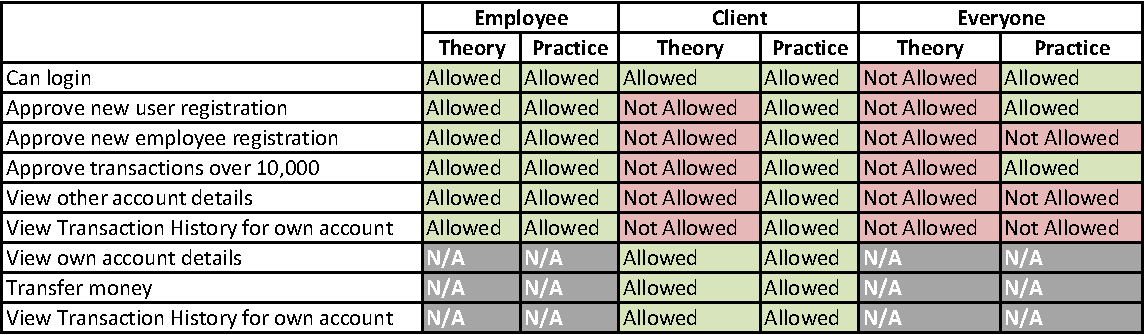
\includegraphics[width=\textwidth]{figures/RoleDefinitionsDoge}
	\caption{Role Definitions}
	\label{figure:RoleDefinitionsDoge}
\end{figure}


\vultable{\gnb}{%
	Clients, Employees and non-logged in users all act as expected, see \ref{figure:RoleDefinitionsGNB}
}{%
	This was verified through basic function testing and security testing tools (ZAP).
}{%
	N/A since no vulnerability was found.
}{%
	N/A 
}{%
\cvssBaseScorePretty{N}{L}{N}{N}{U}{L}{L}{L} %FIXME: This are mock values
}

\begin{figure}[h!tbp]
	\centering
	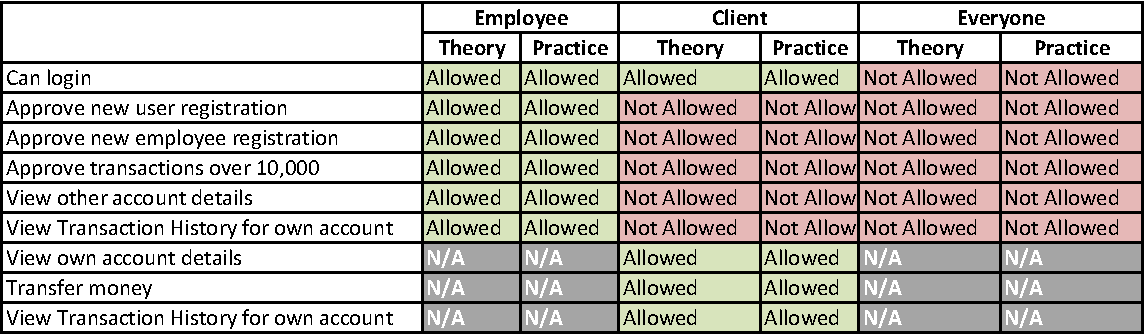
\includegraphics[width=\textwidth]{figures/RoleDefinitionsGNB}
	\caption{Role Definitions}
	\label{figure:RoleDefinitionsGNB}
\end{figure}


\vulntitle{OTG-IDENT-002}{Test User Registration Process}
\vultable{\doge}{%
	The registration process is set up for anyone to register, the process then awaits human interaction for the approval stage, this will serve an extra step of verification.

	Identities are not verified nor checked at this stage due to application limitations, email format verification is missing from the form.
	
	No CAPTCHA or similar tests available to test for human accounts
}{%
	The email verification test was discovered through trail and error while registering.
	Lack of human testing was found through simple observation.
}{%
	likely, due to intentional or unintentional mistyping.
	Robot accounts are less likely to occur and it depends on the skill level of the attacker.
}{%
	No serious impact as TAN codes are not sent to the email.
	Robot accounts can be used to perform a DOS attack. 
}{%
\cvssBaseScorePretty{N}{L}{N}{N}{U}{L}{L}{L} %FIXME: This are mock values
}

\vultable{\gnb}{%
	The registration process is set up for anyone to register, the process then awaits human interaction for the approval stage, this will serve an extra step of verification.
	
	Identities are not verified nor checked at this stage due to application limitations.
	
	No CAPTCHA or similar tests available to test for human accounts.
}{%
	Lack of human testing was found through simple observation.
}{%
	Robot accounts are less likely to occur and it depends on the skill level of the attacker.
}{%
	Robot accounts can be used to perform a DOS attack. 
}{%
\cvssBaseScorePretty{N}{L}{N}{N}{U}{L}{L}{L} %FIXME: This are mock values
}

\vulntitle{OTG-IDENT-003}{Test Account Provisioning Process}
\vultable{\doge}{%
	Provisioning clients is an easy process with no effective mechanisms to verify or vet clients besides a manual approval process.
	
	Vulnerabilities with creating the client account have been discussed in the previous section \ref{vuln:OTG-IDENT-002}, but using Bug No.2 an non-authenticated user is able to approve a client user request.
	
	Provisioning Employees is set up to only be possible by other employees, but using Bug No.12, a non-authenticated user is able to create an employee account.
	%TODO Add bug referencing in this section 
}{%
	This was discovered through trail and error in the bug discovery phase.
}{%
	This vulnerability requires some basic knowledge of the PHP pages and variable names, which can be obtained using basic testing tools, so while this vulnerability is likely to be discovered by an attacker with some basic skills.
}{%
	This presents some serious impact, as creating an employee account will give the attacker full access to the application and administrative functions such as creating accounts and approving money transfers. 
}{%
\cvssBaseScorePretty{N}{L}{N}{N}{U}{L}{L}{L} %FIXME: This are mock values
}

\vultable{\gnb}{%
	Provisioning clients is an easy process with no effective mechanisms to verify or vet clients besides a manual approval process, provisioning Employees is set up in a similar matter.
	
	Vulnerabilities with creating the client account have been discussed in the previous section \ref{vuln:OTG-IDENT-002}, the same applies to creating employee accounts, so a potential DOS attack is possible by creating robot accounts. 
}{%
	This was found through following the given process for creating accounts.
}{%
	Robot accounts are less likely to occur and it depends on the skill level of the attacker.
}{%
	If the DOS attack is severe enough it could stop the application from from working. 
}{%
\cvssBaseScorePretty{N}{L}{N}{N}{U}{L}{L}{L} %FIXME: This are mock values
}

\vulntitle{OTG-IDENT-004}{Testing for Account Enumeration and Guessable User Account}
\vultable{\doge}{%
	Errors provided from enumerating through the different cases are as follows :
	\begin{itemize}
		\item Valid username with correct password : Expected result of logging in 
		\item Valid username with incorrect password : Returns "Username or Password incorrect! Please try again!"
		\item Invalid username : Returns "Username or Password incorrect! Please try again!"
	\end{itemize}
}{%
	This was found through trail and error on different combinations of credentials.
}{%
	\na
}{%
	\na
}{%
	Secure
}

\vultable{\gnb}{%
	Errors provided from enumerating through the different cases are as follows :
	\begin{itemize}
		\item Valid username with correct password: Expected result of logging in 
		\item Valid username with incorrect password: Returns "Invalid login credentials!"
		\item Invalid username : Returns "Invalid login credentials!"
	\end{itemize}
}{%
	This was found through trail and error on different combinations of credentials.
}{%
	\na
}{%
	\na
}{%
	Secure
}

\vulntitle{OTG-IDENT-005}{Testing for Weak or unenforced username policy}
\vultable{\doge}{%
	No username policy applied.
}{%
	\na
}{%
	\na
}{%
	\na
}{%
	\na
}

\vultable{\gnb}{%
	Username has to be in valid email address format.
}{%
	Through trail and error.
}{%
	\na
}{%
	\na
}{%
	Secure. 
}
\newpage
\section{Authentication Testing}	
\simpleVulntitle{OTG-AUTHN-001}{Testing for Credentials Transported over an Encrypted Channel}
\vultable{\doge}{%
	Due to the fact, that no encryption is used when accessing the application, credentials transported over an encrypted channel are vulnerable.
		
	Relevant information regarding unencrypted communication has already been mainly covered in section \ref{vuln:OTG-CRYPST-003} and in \ref{vuln:OTG-CONFIG-007}.				
}{%
	Through observation.
}{%
	Given that a simple network sniffing tracking tool would pick up the credentials, this vulnerability is likely to be exploited.
}{%
	The attacker is able access the said account, and perform actions on behalf of said user, and it the account is an employee account, the attacker would gain access to the administrative tasks
}{%
\cvssBaseScorePretty{N}{L}{N}{N}{U}{L}{L}{L} %FIXME: This are mock values
}

\vultable{\gnb}{%
	\same				
}{%
	\same
}{%
	\same
}{%
	\same 
}{%
\cvssBaseScorePretty{N}{L}{N}{N}{U}{L}{L}{L} %FIXME: This are mock values
}

\vulntitle{OTG-AUTHN-002}{Testing for default credentials}
\vultable{\doge}{%
	The Administrator had a predictable username "employee" and an easy to guess short password "pass".				
}{%
	Credentials were provided in the team report.
}{%
	If an attacker is performing a basic dictionary attack, this vulnerability would very likely be discovered. 
}{%
	Gaining access to the employee account would allow the attacker to perform administrative tasks on the application.	
}{%
\cvssBaseScorePretty{N}{L}{N}{N}{U}{L}{L}{L} %FIXME: This are mock values
}

\vultable{\gnb}{%
	Administrator(Employee) and client users did not have predictable credentials.				
}{%
	Credentials were provided in the team report.
}{%
	\na 
}{%
	\na
}{%
	Secure
}

\vulntitle{OTG-AUTHN-003}{Testing for Weak lock out mechanism}
\vultable{\doge}{%
	No lockout mechanism is deployed. 
}{%
	Through trail and error.
}{%
	This allows for brute force attacks on accounts if the attacker has a username. 
}{%
	Gaining access to an employee or client account, which allow the attacker to perform that accounts tasks.	
}{%
	\cvssBaseScorePretty{N}{L}{N}{N}{U}{L}{L}{L} %FIXME: This are mock values
}

\vultable{\gnb}{%
	\same				
}{%
	\same
}{%
	\same
}{%
	\same
}{%
	\cvssBaseScorePretty{N}{L}{N}{N}{U}{L}{L}{L} %FIXME: This are mock values
}

\vulntitle{OTG-AUTHN-004}{Testing for bypassing authentication schema}
\vultable{\doge}{%
	Through direct page request, parameter modification, and SQL injection a non-authenticated user is able to gain access to both client and employee functions see Bug No.12 and Bug No.2  for more details on how to exploit such bugs, from more details on what is possible, please refer to \ref{figure:RoleDefinitionsDoge}.
	e.g. The url \texttt{/downloadTans.php?userid=1} allows a non authorized user to download the TAN codes for the user with the user id of 1.
	%TODO Add bug referencing in this section 
}{%
	This was discovered through trail and error in the bug discovery phase.
}{%
	This vulnerability requires some basic knowledge of the PHP pages and variable names, which can be obtained using basic testing tools, so while this vulnerability is likely to be discovered by an attacker with some basic skills.
}{%
	This presents some serious impact, as creating an employee account will give the attacker full access to the application and administrative functions such as creating accounts and approving money transfers. 	
}{%
\cvssBaseScorePretty{N}{L}{N}{N}{U}{L}{L}{L} %FIXME: This are mock values
}

\vultable{\gnb}{%
	The PHP Session ID cookie variable is not destroyed after logout, and even though the user is unable to use the "back" option on the browser, the PHP Session ID does not change though making it extremely predictable after logging 
}{%
	This was done through cookie inspection using the chrome and Firefox Developer extensions.
}{%
	The skill level required for exploiting this is minimal, Knowledge needed for this attack is basic cookie inspection and injection and Network sniffing.
}{%
	Overtake an existing user session and gain access to that users privileges.
}{%
	\cvssBaseScorePretty{N}{L}{N}{N}{U}{L}{L}{L} %FIXME: This are mock values
}

\vulntitle{OTG-AUTHN-005}{Test remember password functionality}
\vultable{\doge}{%
	Passwords in this application are sent in clear text.
}{%
	Through HTTP Header inspection
}{%
	The skill level required for exploiting this is minimal, Knowledge needed for this attack is basic HTTP Header inspection and Network sniffing.
}{%
	Gaining access to an employee or client account, which allow the attacker to perform that accounts tasks.	
}{%
	\cvssBaseScorePretty{N}{L}{N}{N}{U}{L}{L}{L} %FIXME: This are mock values
}

\vultable{\gnb}{%
	\same				
}{%
	\same
}{%
	\same
}{%
	\same
}{%
	\cvssBaseScorePretty{N}{L}{N}{N}{U}{L}{L}{L} %FIXME: This are mock values
}


\vulntitle{OTG-AUTHN-006}{Testing for Browser cache weakness}
\vultable{\doge}{%
	Browser Cache settings are set up correctly, so 'Back' on the browser does not work.
}{%
	Though observation.
}{%
	\na
}{%
	\na	
}{%
	Secure
}

\vultable{\gnb}{%
	\same				
}{%
	\same
}{%
	\same
}{%
	\same
}{%
	\same
}


\vulntitle{OTG-AUTHN-007}{Testing for Weak password policy}
\vultable{\doge}{%
	No password policy is implemented.
}{%
	Though observation.
}{%
	The skill level required for exploiting a week password is minimal,  either through password cracking tools or social engineering.
}{%
	Gaining access to an employee or client account, which allow the attacker to perform that accounts tasks.	
}{%
\cvssBaseScorePretty{N}{L}{N}{N}{U}{L}{L}{L} %FIXME: This are mock values
}

\vultable{\gnb}{%
	\same				
}{%
	\same
}{%
	\same
}{%
	\same
}{%
	\cvssBaseScorePretty{N}{L}{N}{N}{U}{L}{L}{L} %FIXME: This are mock values
}


%\vulntitle{OTG-AUTHN-008}{Testing for Weak security question/answer}
%\vulntitle{OTG-AUTHN-009}{Testing for weak password change or reset functionalities}
%\vulntitle{OTG-AUTHN-010}{Testing for Weaker authentication in alternative channel}

\newpage
\section{Authorization Testing}

\simpleVulntitle{OTG-AUTHZ-001}{Testing Directory traversal/file include}
\vultable{\doge}{%
	No user defined input vectors to include additional files were discovered during testing.
}{%
	After capturing the requests and responses of all pages available in the application with Zed Attack proxy, the recorded traffic was checked for possible input vectors.
	No input vectors referencing files were found.
}{%
	\na
}{%
	\na
}{%
	\na
}
\vultable{\gnb}{%
	User defined input vectors were observed on all pages of the application which require authentication.
	These input vectors don't seem to be direct references to files in the wep application, thus an indirect mapping of the specified names to included files is assumed.
	Due to this indirect mapping accessing arbitrary files on the server is not possible by modifying these input vectors.
	Nevertheless an authenticated attacker is able to use this mechanism to get access to all included pages as described in \vulnref{OTG-AUTHZ-002}
}{%
	After capturing the requests and responses of all pages available in the application with Zed Attack proxy, the recorded traffic was checked for possible input vectors.
	Multiple input vectors referencing sections of the site were identified, but manual testing revealed that none of these referred to filenames directly.
}{%
	See \vulnref{OTG-AUTHZ-002}
}{%
	See \vulnref{OTG-AUTHZ-002}
}{%
	See \vulnref{OTG-AUTHZ-002}
}

\vulntitle{OTG-AUTHZ-002}{Testing for bypassing authorization schema}
\vultable{\doge}{%
	All employee pages are fully accessible for any authenticated user e.g. client.
}{%
	Manually accessing the address of the employee pages while being logged in as user allowed full access to these sites.
	\texttt{http://ADDRESS/employee\_home.php}
}{%
	To exploit this vulnerability an attacker needs to be aware of the address of the employee pages and have an valid client account.
}{%
	This vulnerability allows bypassing all authorization mechanisms put in place, granting the attacker the highest privileges available in the application.
}{%
	\cvssBaseScorePretty{N}{L}{N}{N}{C}{L}{L}{L} %FIXME: This are mock values
}
\vultable{\gnb}{%
	Direct access to the employee page is not possible as client.
	However by using the file inclusion technique described in \vulnref{OTG-AUTHZ-001} an authenticated attacker is able to access all included pages of the application.
}{%
	Manual testing direct access to the employee pages (\texttt{http://ADDRESS/employee/employee.php}) did not grant any positive results.\newline 
	Using the information gathered in \vulnref{OTG-AUTHZ-001} it was possible to access the employee pages by modifying the POST parameters of the client page to reference the employee pages.
	Page: \texttt{http://ADDRESS/client/client.php}\newline
	Original POST parameters:\newline
	\texttt{section=my\_accounts\&frame=account\_overview\&account=10000002}\newline
	Updated POST parameters:\newline
	\texttt{section=employee\_area\&frame=manage\_registration}\newline
	This opened the page with pending registrations which should only be visible as employee.
	Additional effort is required to start any further actions from this page (e.g.\ approving users) as the required javascript is missing and all references lead to the wrong page.
	The same applies for all other employee pages.
}{%
	To access these sites an attacker has to be authenticated and aware of the names of the employee pages.
	As the client area pages doesn't contain the required javascript code for the employee area, additional knowledge and effort is required to perform actions on the pages accessed by this method.
}{%
	This vulnerability allows bypassing all authorization mechanisms put in place, granting the attacker the highest privileges available in the application.
}{%
	\cvssBaseScorePretty{N}{L}{N}{N}{C}{L}{L}{L} %FIXME: This are mock values
}

\vulntitle{OTG-AUTHZ-003}{Testing for Privilege Escalation}
\vulntitle{OTG-AUTHZ-004}{Testing for Insecure Direct Object References}

\newpage
\section{Session Management Testing}
%SESSION 001
\simpleVulntitle{OTG-SESS-001}{Testing for Bypassing Session Management Schema}
\vultable{\doge}{%
	When accessing the application, a randomly generated PHPSESSID session cookie is set. The cookie doesn't have an expiration date nor is it tagged as secure. Apparently the session cookie is already set before logging into the application. This cookie is simply replaced by a new one once the user logs out of the application. No other cookies are set. Also if the cookie is tampered with, the server automatically generates a new cookie, containing a new session ID.
}{%
	The PHPSESSID cookie has been discovered while intercepting HTTP requests/responses using Burp. The same cookie details were later on confirmed using the Cookies plugin for browser.
}{%
	\na
}{%
	Since the only used cookie only contains the session ID, even though it is easy to change the value of the cookie, no other session values are exposed to the user. It is still possible to hijack another session by changing the entire value of the cookie with the one associated to another user (see Session 004).
}{%
\na
}
\vultable{\gnb}{%
	The same observations made for the DogeBank application apply.
}{%
	The PHPSESSID cookie was analyzed using the Cookies plugin for browser.
}{%
	\na
}{%
	The same implications mentioned for the DogeBank application apply.
}{%
\na
}
%SESSION 002
\vulntitle{OTG-SESS-002}{Testing for Cookies attributes}
\vultable{\doge}{%
	We found that the cookie generated by the application does NOT set the following attributes:
	\begin{itemize}
		\item Secure
		\item HttpOnly
		\item Expires
	\end{itemize}
	The application also sets the domain attribute very loosely, since the path is set to the root directory "/".
}{%
	The attributes were analyzed using the Cookies plugin for browser.
}{%
	It is easy to access the cookies from Javascript, as long as the browser supports client-side scripting.
}{%
	Weak protection for cookies means that these can be accessed via Javascript to perform XSS attacks.
}{%
\cvssBaseScorePretty{N}{L}{N}{N}{U}{L}{L}{L} %FIXME: This are mock values
}
\vultable{\gnb}{%
	The same observations made for the DogeBank application apply.
}{%
	The attributes were analyzed using the Cookies plugin for browser.
}{%
	It is easy to access the cookies from Javascript, as long as the browser supports client-side scripting.
}{%
	Weak protection for cookies means that these can be accessed via Javascript to perform XSS attacks.
}{%
\cvssBaseScorePretty{N}{L}{N}{N}{C}{L}{L}{L} %FIXME: This are mock values
}
%SESSION 003
\vulntitle{OTG-SESS-003}{Testing for Session Fixation}
\vultable{\doge}{%
	After careful observation and testing we found that once a session ID has been set, this will not be changed until a user logs out. More specifically, the session ID will not be invalidated before a login operation, remaining the same after having logged in (a session ID is generated on the login page already).
}{%
	The session ID generation was thoroughly observed thanks to a Proxy that intercepted all GET/POST requests and responses to/from the server. For this the Burp Suite tool was used.
}{%
	Setting up a possible attack is theoretically easy, but it requires a victim to be tricked by the attacker, making the attack less likely depending on the victim.
}{%
	An attacker could generate a session ID for himself, then force the same ID onto a user, hijacking that users' session in case of successful authentication with the server. This implicates full access to the account of a user.
}{%
\cvssBaseScorePretty{N}{L}{N}{N}{U}{L}{L}{L} %FIXME: This are mock values
}
\vultable{\gnb}{%
	The same observations made for the DogeBank application apply.
}{%
	The discovery was made thanks to GET/POST requests interception.
}{%
	The same likelihood described for the DogeBank application applies.
}{%
	The same implications mentioned for the DogeBank application apply.
}{%
\cvssBaseScorePretty{N}{L}{N}{N}{C}{L}{L}{L} %FIXME: This are mock values
}
%SESSION 004
\vulntitle{OTG-SESS-004}{Testing for Exposed Session Variables}
\vultable{\doge}{%
	After observing requests and responses between the client and the server, we observed that session IDs are always sent in HTTP headers. Although the session ID is never explicitly passed in URLs, no encryption is provided whatsover and the session ID does not change until a user explicitly logs out. No other session variables are generated, therefore only the session ID is affected.
}{%
	This observation was made when analyzing session management. Refer to Section 001, 003.
}{%
	As long as an attacker can sniff the network traffic and read the session ID of a user, it is very easy to hijack a session. This approach makes it even easier than hijacking a session through social engineering.
}{%
	An attacker can perform a man in the middle attack, read the unencrypted HTTP messages exchanged between a user and the server, in order to impersonate the user and hijack an existing session. This implicates full access to the account of a user.
}{%
\cvssBaseScorePretty{N}{L}{N}{N}{U}{L}{L}{L} %FIXME: This are mock values
}
\vultable{\gnb}{%
	The same observations made for the DogeBank application apply.
}{%
	The discovery was made thanks to GET/POST requests interception.
}{%
	The same likelihood described for the DogeBank application applies.
}{%
	The same implications mentioned for the DogeBank application apply.
}{%
\cvssBaseScorePretty{N}{L}{N}{N}{C}{L}{L}{L} %FIXME: This are mock values
}
%SESSION 005
\vulntitle{OTG-SESS-005}{Testing for Cross Site Request Forgery}
\vultable{\doge}{%
	Having observed different functionalities offered by the server, we noticed that no encryption is used at all; furthermore the session ID is stored as a cookie in the browser of the user, which makes things a lot easier. In order to trick a user into execute specific operations, however, we found out that some knowledge of the web application was required. Given this knowledge, it proves easy to compromise the entire web application. We found a list of pages potentially subject to CSRF:
	\begin{itemize}
		\item approveuser.php: can be exploited without privileges as well;
		\item approvetransaction.php: can be exploited without privileges as well;
		\item downloadTans.php: can be exploited without privileges as well;
		\item register\_employee.php: only accessible to employees. The existence of this page has to be known to an attacker beforehand;
		\item tran.php: although this page is easy to exploit, an attacker would need to have access to the TANs of a user. This could be done beforehand by downloading from \url{http://ADDRESS/downloadTans.php}.
	\end{itemize}
}{%
	All of the observations were made while navigating the website and brute-forcing different combinations of attacks. Other helpful tools helpful were DirBuster and the DogeBankHack custom script, since these allowed to gain a better understanding of the website's structure.
}{%
	In theory, performing a CSRF attack would be easy, since session IDs are stored in browsers and sent over unencrypted channels. However, in this specific case, the attack complexity increases, since the attacker requires additional knowledge, like the ID of a user and the names of the vulnerable pages. In most of the above mentioned cases, getting access to the ID of a user proves to be trivial, since it is contained in pages shown to the user (easy to exploit via Javascript).
}{%
	An attacker in possession of the previously described information could be able to trick a victim into executing operations predetermined by the attacker himself, like starting transactions to arbitrary accounts or registering arbitrary employees. The impact in the former case would compromise the whole bank account of a user, or grant a privilege escalation in the latter case.
}{%
\cvssBaseScorePretty{N}{L}{N}{N}{U}{L}{L}{L} %FIXME: This are mock values
}
\vultable{\gnb}{%
	The same predisposition showed by the DogeBank application holds true, i.e. no encryption is used in client-server message exchanges and the session ID is stored as a cookie in the browser of the user. Similar observations regarding the knowledge required to perform a CSRF attack also hold. In particular, these pages proved to be vulnerable:
	\begin{itemize}
		\item verify\_transaction.php: as for the DogeBank case, an attacker would need to have access to the TANs of a user in order to exploit this page. Getting access to these TANs, however, is only possible by either accessing the database directly or intercepting the confirmation email sent to a user;
		\item manage\_registration.php: requires knowledge of the ID of the user that we want to approve/reject. Other than that, exploiting this page proved to be trivial and just required a proper analysis of the client-side code;
		\item manage\_transfer.php: this page is also easy to exploit, since it only requires knowledge of the pending transactions IDs, which can be found on the same page;
		\item manage\_clients.php: although this page can be accessed directly, its existence has to be known to the attacker.
	\end{itemize}
	It is important to stress that, given the layout of the pages, the above mentioned pages can simply be used as section parameters inside a POST request to the employee.php and client.php pages, without the need to copy additional Javascript from the container pages.
}{%
	These observations were made while navigating the website and brute-forcing different combinations of attacks.
}{%
	As for the DogeBank case, although a CSRF attack would be easy, the complexity increases in this specific case, since an attacker needs some knowledge about the layout of the pages (i.e. the names of the above mentioned vulnerable php sections). This information is harder to acquire than in the previous case however, as it required a thorough client-side code analysis.
}{%
	Assuming an attacker is capable of obtaining the required information for such an attack to work, this would have the same implications described in the DogeBank case.
}{%
\cvssBaseScorePretty{N}{L}{N}{N}{C}{L}{L}{L} %FIXME: This are mock values
}
%SESSION 006
\vulntitle{OTG-SESS-006}{Testing for logout functionality}
\vultable{\doge}{%
	We observed that the logout functionality is working properly, as the logoutAction.php destroys an existing session, creating a new one. Trying to access a page that requires authentication, after having logged out, fails and the server responds with a "PHPSESSID=deleted" cookie, redirecting the browser to the login page.
	We also observed that there is no logout timer, allowing a user to be logged in indefinetely, as long as the logout is not manually triggered.
}{%
	These observations were made using the Burp Repeater tool.
}{%
	\na
}{%
	Since there is no session timeout policy whatsoever, this could prove to be a vulnerability. This is analyzed in more details in SESS-007
}{%
\cvssBaseScorePretty{N}{L}{N}{N}{U}{L}{L}{L} %FIXME: This are mock values
}
\vultable{\gnb}{%
	The same observations made for the DogeBank application apply.
}{%
	These observations were made using the Burp Repeater tool.
}{%
	\na
}{%
	The same implications described for the DogeBank application apply.
}{%
\cvssBaseScorePretty{N}{L}{N}{N}{C}{L}{L}{L} %FIXME: This are mock values
}
%SESSION 007
\vulntitle{OTG-SESS-007}{Test Session Timeout}
\vultable{\doge}{%
	We observed that no session timeout policy was implemented, neither on server side nor on client side. Although the only sensitive information stored on client side is the session ID, we proved that it was possible to reuse the same session any number of times.
}{%
	These observations were made using the Burp Repeater tool.
}{%
	A session hijacking is easy to perform, as long as the attacker can either sniff the traffic between the victim and the server, or has access to the device from which the victim logged in.
}{%
	The lack of a session timeout gives a potential attacker indefinite time to perform a session hijacking. Once a session has been hijacked, an attacker has complete access over a user's account.
}{%
\cvssBaseScorePretty{N}{L}{N}{N}{U}{L}{L}{L} %FIXME: This are mock values
}
\vultable{\gnb}{%
	The same observations made for the DogeBank application apply.
}{%
	These observations were made using the Burp Repeater tool.
}{%
	The same likelihood described for the DogeBank application applies.
}{%
	The same implications mentioned for the DogeBank application apply.
}{%
\cvssBaseScorePretty{N}{L}{N}{N}{C}{L}{L}{L} %FIXME: This are mock values
}
%SESSION 008
\vulntitle{OTG-SESS-008}{Testing for Session puzzling}
\vultable{\doge}{%
	Considering that the only session variable set by the application is the session ID, which we observed is randomly generated by the server, there isn't really any margin for session variable overloading.
}{%
	These observations were made using the Burp suite tool.
}{%
	\na
}{%
	\na
}{%
	Secure
}
\vultable{\gnb}{%
	The same observations made for the DogeBank application apply.
}{%
	These observations were made using the Burp suite tool.
}{%
	\na
}{%
	\na
}{%
	Secure
}

\newpage
\section{Data Validation Testing}
\simpleVulntitle{OTG-INPVAL-001}{Testing for Reflected Cross Site Scripting}
\vulntitle{OTG-INPVAL-002}{Testing for Stored Cross Site Scripting}
\vulntitle{OTG-INPVAL-003}{Testing for HTTP Verb Tampering}
\vulntitle{OTG-INPVAL-004}{Testing for HTTP Parameter pollution}
\vulntitle{OTG-INPVAL-005}{Testing for SQL Injection}
\vulntitle{OTG-INPVAL-006}{Testing for LDAP Injection}
\vulntitle{OTG-INPVAL-007}{Testing for ORM Injection}
\vulntitle{OTG-INPVAL-008}{Testing for XML Injection}
\vulntitle{OTG-INPVAL-009}{Testing for SSI Injection}
\vulntitle{OTG-INPVAL-010}{Testing for XPath Injection}
\vulntitle{OTG-INPVAL-011}{IMAP/SMTP Injection}

\vulntitle{OTG-INPVAL-012}{Testing for Code Injection}
\vultable{\doge}{%
	This vulnerability is not applicable due to the fact that none of the pages of the \doge{} allows to provide a parameter that will be executed. See~\ref{vuln:OTG-INPVAL-013} for a similiar attack using the filename of the uploaded batch transactions file.
}{%
	This was observed using a Proxy that intercepted all GET/POST requests and responses to/from the server. For this the Burp Suite tool was used.
}{%
	\na
}{%
	\na
}{%
	\naScore
}
\vultable{\gnb}{%
	This vulnerability is not applicable due to the fact that none of the pages of the \gnb{} allows to provide a parameter that will be executed.
}{%
	This was observed using a Proxy that intercepted all GET/POST requests and responses to/from the server. For this the Burp Suite tool was used.
}{%
	\na
}{%
	\na
}{%
	\naScore
}

\vulntitle{OTG-INPVAL-012-1}{Testing for Local File Inclusion}
\vultable{\doge}{%
	This vulnerability is not applicable due to the fact that none of the pages of the \doge{} allows to provide a parameter specifying files.
}{%
	This was observed using a Proxy that intercepted all GET/POST requests and responses to/from the server. For this the Burp Suite tool was used.
}{%
	\na
}{%
	\na
}{%
	\naScore
}
\vultable{\gnb}{%
	This vulnerability is not applicable due to the fact that none of the pages of \gnb{} allows to provide a parameter specifying files. The \gnb{} can be exploited though by messing with the internal lookup that gets the php filename from a keyword. See~\ref{vuln:OTG-AUTHZ-001} for a more detailed description.
}{%
	This was observed using a Proxy that intercepted all GET/POST requests and responses to/from the server. For this the Burp Suite tool was used.
}{%
	\na
}{%
	\na
}{%
	\naScore
}

\vulntitle{OTG-INPVAL-012-2}{Testing for Remote File Inclusion}
\vultable{\doge}{%
	This vulnerability is not applicable due to the fact that none of the pages of \doge{} allows to provide a parameter specifying files.
}{%
	This was observed using a Proxy that intercepted all GET/POST requests and responses to/from the server. For this the Burp Suite tool was used.
}{%
	\na
}{%
	\na
}{%
	\naScore
}
\vultable{\gnb}{%
	\same
}{%
	\same
}{%
	\na
}{%
	\na
}{%
	\naScore
}

\vulntitle{OTG-INPVAL-013}{Testing for Command Injection}
\vulntitle{OTG-INPVAL-014}{Testing for Buffer overflow}
Testing for Heap overflow\\
Testing for Stack overflow\\
Testing for Format string\\
\vulntitle{OTG-INPVAL-015}{Testing for incubated vulnerabilities}
\vulntitle{OTG-INPVAL-016}{Testing for HTTP Splitting/Smuggling}

\newpage
\section{Error Handling}
\simpleVulntitle{OTG-ERR-001}{Analysis of Error Codes}
\vulntitle{OTG-ERR-002}{Analysis of Stack Traces}

\newpage
\section{Cryptography}
\simpleVulntitle{OTG-CRYPST-001}{Testing for Weak SSL/TSL Ciphers, Insufficient Transport Layer Protection}
\vultable{\doge}{%
	Due to the fact, that the application is only accessible via HTTP and no SSL/TLS encryption is used no testing for weak ciphers could be performed.
	Relevant information leakage resulting from the unencrypted communication has already been covered in \vulnref{OTG-CONFIG-007} and \vulnref{OTG-CRYPST-003}.
}{%
	\na
}{%
	\na
}{%
	\na
}{%
	\na
}
\vultable{\gnb}{%
	The same observations made for the DogeBank application apply.
	Relevant information leakage resulting from the unencrypted communication has already been covered in \vulnref{OTG-CONFIG-007} and \vulnref{OTG-CRYPST-003}.
}{%
	\na
}{%
	\na
}{%
	\na
}{%
	\na
}

\vulntitle{OTG-CRYPST-002}{Testing for Padding Oracle}
\vultable{\doge}{%
	Due to the fact, that no encryption is used when accessing the application, no padding of information is used.
	Relevant information leakage resulting from the unencrypted communication has already been covered in \vulnref{OTG-CONFIG-007} and \vulnref{OTG-CRYPST-003}.
}{%
	\na
}{%
	\na
}{%
	\na
}{%
	\na
}
\vultable{\gnb}{%
	The same observations made for the DogeBank application apply.
	Relevant information leakage resulting from the unencrypted communication has already been covered in \vulnref{OTG-CONFIG-007} and \vulnref{OTG-CRYPST-003}.
}{%
	\na
}{%
	\na
}{%
	\na
}{%
	\na
}

\vulntitle{OTG-CRYPST-003}{Testing for Sensitive information sent via unencrypted channels}
\vultable{\doge}{%
	Sensitive information is sent over unencrypted channels in every request the user performs as the application is only accessible via HTTP and no SSL/TLS encryption is used.
}{%
	As documented in \vulnref{OTG-CONFIG-007}, the site is not available via HTTPS.
}{%
	Every requests gets sent over an unecrypted channel automatically.
}{%
	The same implications as in \vulnref{OTG-CONFIG-007} apply.
	By sniffing the network traffic, all data exchanged between the server and the client can be read as clear text. No confidentiality at all is supported on this end.
}{%
	\cvssBaseScorePretty{N}{L}{N}{N}{U}{L}{L}{L} %FIXME: This are mock values
}
\vultable{\gnb}{%
	\same
}{%
	\same
}{%
	\same
}{%
	\same
}{%
	\cvssBaseScorePretty{N}{L}{N}{N}{U}{L}{L}{L} %FIXME: This are mock values
}

\newpage
\section{Business Logic Testing}
\simpleVulntitle{OTG-BUSLOGIC-001}{Test Business Logic Data Validation}
\vulntitle{OTG-BUSLOGIC-002}{Test Ability to Forge Requests}
\vulntitle{OTG-BUSLOGIC-003}{Test Integrity Checks}
\vulntitle{OTG-BUSLOGIC-004}{Test for Process Timing}
\vulntitle{OTG-BUSLOGIC-005}{Test Number of Times a Function Can be Used Limits}
\vulntitle{OTG-BUSLOGIC-006}{Testing for the Circumvention of Work Flows}
%BUSLOGIC 007
\vulntitle{OTG-BUSLOGIC-007}{Test Defenses Against Application Mis-use}
\vultable{\doge}{%
	After thorough testing and observation we concluded that no mechanisms to prevent against application mis-use are in place. No critical functionalities are disabled and no logs are kept.
}{%
	These observations were made after using several different tools and manually stress-testing the application.
}{%
	\na
}{%
	This vulnerability implicates that an attacker will be able to attempt countless attacks and abuse functionalities without any repercussion.
}{%
\cvssBaseScorePretty{N}{L}{N}{N}{U}{L}{L}{L} %FIXME: This are mock values
}
\vultable{\gnb}{%
	The same observations made for the DogeBank application apply.
}{%
	These observations were made after using several different tools and manually stress-testing the application.
}{%
	\na
}{%
	The same implications mentioned for the Doge application apply.
}{%
\cvssBaseScorePretty{N}{L}{N}{N}{U}{L}{L}{L} %FIXME: This are mock values
}
%BUSLOGIC 008
\vulntitle{OTG-BUSLOGIC-008}{Test Upload of Unexpected File Types}
\vultable{\doge}{%
	We discovered that the tran.php page allows to upload any kind of file, without performing extension checks on it. However, it seems that the server accepts only files with a limited size, making it impossible to generate more than 3 transactions at once, or uploadin huge files for that matter. Regardless, as long as the filesize stays below 500 bytes, any file will be accepted by the server and stored forever inside the /uploads folder.
}{%
	It is important to stress that no file format was described on the documentation nor on the transaction page. Nonetheless, after having found out the structure of the web application (using DirBuster and Burp), we found a sample batch transaction file in txt format. Afterwards we simply tried uploading files with different extensions to see the outcome.
}{%
	The likelihood of a an attacker uploading a file with a bad filename or a non-expected extension is very high.
}{%
	This was by far the most severe vulnerability we found, since all uploaded files are kept inside a well known folder on the web server. An attacker is this way able to upload any file, as well as custom scripts and programs to the server. This issue is analyzed in depth in section 009.
}{%
\cvssBaseScorePretty{N}{L}{N}{N}{U}{L}{L}{L} %FIXME: This are mock values
}
\vultable{\gnb}{%
	The only page which allows to upload a file to the server is the new\_transaction\_multiple.php (loaded as a frame under the my\_accounts.php section inside the client.php file). When uploading a file, the server performs an explicit check, eventually accepting only .csv and .txt files.
}{%
	We tried uploading several files with different file extensions, leading to the result described above.
}{%
	\na
}{%
	\na
}{%
	Secure
}
%BUSLOGIC 009
\vulntitle{OTG-BUSLOGIC-009}{Test Upload of Malicious Files}
\vultable{\gnb}{%
	Once discovered that the tran.php page allowed to upload any kind of file, we did multiple tests and finally observed that it was indeed possible to upload malicious code. This vulnerability was used to execute both arbitrary C code and custom PHP scripts. Although eventually we gained full access to the application, including credentials, database access and source code, we couldn't tamper too much with the operating system since we didn't have root access.
}{%
	This discovery is a corollary of the one made in section 008. All the attacks performed exploiting this vulnerability were manual attempts.
}{%
	Once an attacker asserted the possibility of uploading any kind of file, the likelihood of such an attack becomes very high.
}{%
	As stated in the BUSLOGIC 008 section, this was the most severe vulnerability found, since it allows to get full control over the application.
	We tried multiple attacks, all of which worked without flawlessly:
	\begin{itemize}
		\item Upload a file which contained malicious code in its filename. The server would simply execute this inside the batch parser and output the results to tran.php page;
		\item Upload a php script which allowed us to start a reverse shell attack.
		\item Upload an interactive php script which could allow us to upload compiled code and execute it.
		\item Upload a php script which could make us tamper with the database
	\end{itemize}
}{%
	\cvssBaseScorePretty{N}{L}{N}{N}{U}{L}{L}{L} %FIXME: This are mock values
}
\vultable{\gnb}{%
	Although the application performs a check on the extension of the file uploaded via the new\_transaction\_multiple.php page, we still managed to upload malicious code by inserting shell commands inside the filename. Since the application only accepts txt and csv files, we simply appended \#.txt at the end of the bad filename.
}{%
	This discovery was made thanks to manual attempts to perform code injection.
}{%
	The likelihood of an attacker attempting a code injection through a file upload is very high.
}{%
	The implications of a code injection attack are very severe, since an attacker could execute arbitrary code on the webserver. Even reading source code becomes possible.
}{%
	\cvssBaseScorePretty{N}{L}{N}{N}{U}{L}{L}{L} %FIXME: This are mock values
}

\newpage
\section{Client Side Testing}
This section was prioritized as low, therefore the client side was not tested in depth. Furthermore, as stated in the OWASP testing guide, black box testing of the client side is usually not performed, since access to the source code is always available, as it needs to be sent to the client to be executed.

\simpleVulntitle{OTG-CLIENT-001}{Testing for DOM based Cross Site Scripting}
\simpleVulntitle{OTG-CLIENT-002}{Testing for JavaScript Execution}
\simpleVulntitle{OTG-CLIENT-003}{Testing for HTML Injection}
\simpleVulntitle{OTG-CLIENT-004}{Testing for Client Side URL Redirect}
\simpleVulntitle{OTG-CLIENT-005}{Testing for CSS Injection}
\simpleVulntitle{OTG-CLIENT-006}{Testing for Client Side Resource Manipulation}
\simpleVulntitle{OTG-CLIENT-007}{Test Cross Origin Resource Sharing}
\simpleVulntitle{OTG-CLIENT-008}{Testing for Cross Site Flashing}
%CLIENT 009
\simpleVulntitle{OTG-CLIENT-009}{Testing for Clickjacking}
\vultable{\doge}{%
	We observed that it is entirely possible to load all of the pages inside
}{%
	This discovery required manual testing: an html with a simple iframe was included, that could contain any of the pages of the the web application.
}{%
	Considering there is not protection against clickjacking attacks whatsoever, this kind of attack could prove to be quite easy.
}{%
	The Doge web application is entirely vulnerable to clickjacking attacks and an attacker could handle all of the actions started on the php pages in a malicious way.
}{%
\cvssBaseScorePretty{N}{L}{N}{N}{U}{L}{L}{L} %FIXME: This are mock values
}
\vultable{\gnb}{%
	The same observations made for the DogeBank application apply.
}{%
	This discovery required manual testing: an html with a simple iframe was included, that could contain any of the pages of the the web application.
}{%
	The same likelihood described for the DogeBank application applies.
}{%
	The GNB web application is entirely vulnerable to clickjacking attacks and an attacker could handle all of the actions started on the php pages in a malicious way.
}{%
\cvssBaseScorePretty{N}{L}{N}{N}{C}{L}{L}{L} %FIXME: This are mock values
}
%CLIENT 010
\simpleVulntitle{OTG-CLIENT-010}{Testing WebSockets}
\vultable{\doge}{%
	The Doge Web Application does not make use of any asynchronous operation, neither using AJAX nor using WebSockets.
}{%
	We asserted that there was no WebSockets communication at all while surfing the pages of the application and testing out all of the functionalities. This was done using Google Chrome's Developer Tools.
}{%
	\na
}{%
	\na
}{%
	Secure
}
\vultable{\gnb}{%
	Although the application makes use of asynchronous requests for the client search functionality, this is done using traditional AJAX and not HTML5 WebSockets. Hence, the application is secure against attacks on WebSockets.
}{%
	To prove our observation, we used Google Chrome's Developer Tools to assert there was no ongoing WebSocket communication when executing search requests.
}{%
	\na
}{%
	\na
}{%
	Secure
}
%CLIENT 011
\simpleVulntitle{OTG-CLIENT-011}{Test Web Messaging}
\simpleVulntitle{OTG-CLIENT-012}{Test Local Storage}
